\section{Print Controls}

\subsection{Approach}
There are many ways to create an FDM 3D printer, as seen in the many models available on the market, from industry-serving companies like Stratasys\footnote{\url{http://www.stratasys.com/}} and 3D Systems\footnote{\url{http://www.3dsystems.com/}} to home printer startups like Makerbot\footnote{\url{http://www.makerbot.com/}} to the many open-source efforts, notably the RepRap\footnote{\url{http://reprap.org/}} ecosystem. Most of these printers operate on Cartesian-style gantry system with 3 degrees of freedom. Some curved-layer printing is attainable on such printers, but the fixed attitude of the print heads limits the layer geometries to those that are accessible from one approach angle. To get around this limitation, a 6-degree-of-freedom robotic arm from FANUC\footnote{\url{http://www.fanucamerica.com/}} was used for this project. In addition to providing the 6 degrees of freedom necessary for curved-layer printing, the robot also provides 0.02mm of positioning repeatibility, which is small with respect to typical FDM nozzle outlet diameters (0.2-0.4mm). The robot was purchased in 2010 in the iRVision package as part of the CERT Program from FANUC. See the program brochure in Section~\ref{sec:cert-brochure} for more details.

Once the robot was chosen as the printing platform, much of the remaining 3D printing toolchain was filled in with parts and software from the RepRap community. These included the extruder hot-end and some related control hardware and software. Some additional control components were purchased from FANUC or fabricated in-house.

\subsection{Overview}
Figure~\ref{fig:sys-overview} gives a schematic overview of the mechanical, hardware, and software components that make up the curved-layer 3D printer system. The robot arm is the mechanical platform for the 3D printer. The custom extruder is fitted to the end of the robot arm and acts as a printing end effector. The motion of the robot arm is controlled by the robot controller, which is programmed by writing TP programs via the controller teach pendant. The extruder hardware, including the heater cartridge, cooling fan, and extrusion motor are controlled by an open-source Megatronics board loaded with the (also open-source) Marlin\footnote{\url{http://reprap.org/wiki/Marlin}} firmware. 

Normally, the Megatronics board is used to control the path of the extruder as well as the extrusion feed rate; the Marlin firmware can thus adjust the extruder filament feedrate according to the surface speed of the extruder in order to maintain the desired volumetric flow rate of hot plastic. However, in this case, the extruder path is controlled by the robot controller, so the extrusion control is independent of the motion control. Ideally, the two systems would be interfaced to allow the robot controller to give look-ahead speed predictions to the extruder controller to allow for tight synchronization. However, the FANUC controller interface only allows such interfacing with approved machinery. The next best option was to add I/O hardware to the FANUC controller and output an analog robot speed signal to the extruder controller. This way, the extruder controller might be able to extrude filament reasonably close to the actual extruder speed by tracking the robot speed output.

\begin{figure}
    \centering
    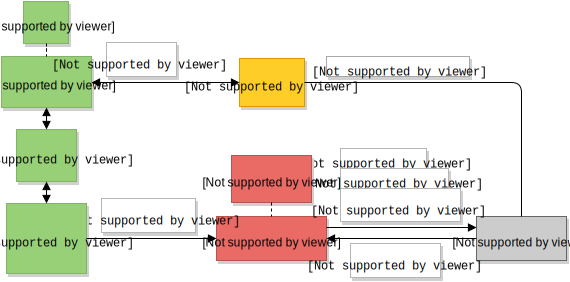
\includegraphics[width=.8\linewidth]{figures/diagrams/system overview}
    \caption{Overview of the 3D printer controls.}
    \label{fig:sys-overview}
\end{figure}

A more detailed electrical schematic is shown in Figure~\ref{fig:schem-fig}. 

\begin{figure}
    \centering
    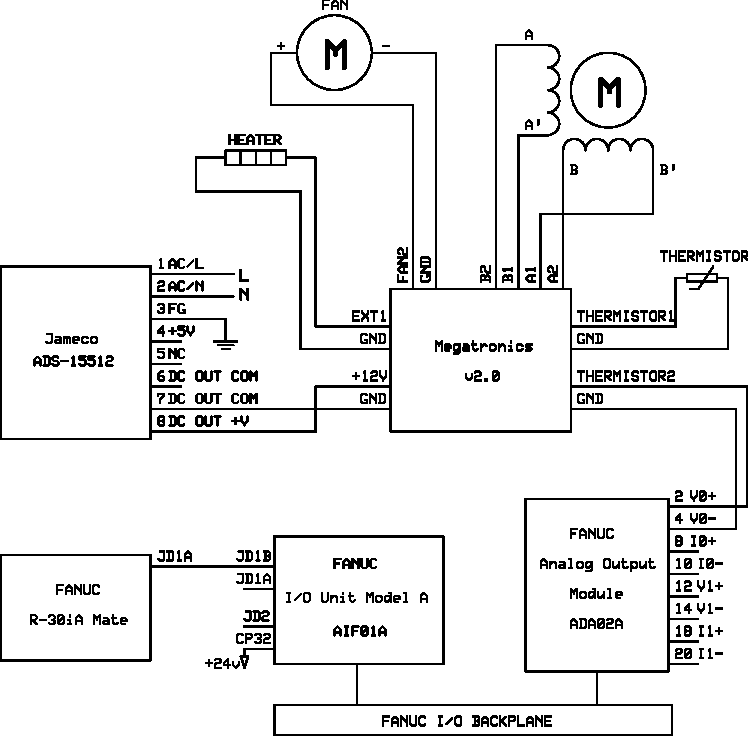
\includegraphics[width=.8\linewidth]{figures/diagrams/schematic-figure}
    \caption{Electrical schematic of the 3D printer controls.}
    \label{fig:schem-fig}
\end{figure}


\subsection{FANUC I/O interface}
The FANUC robot controller makes digital and analog electrical signals available to the user through the teach pendant interface \cite[sec~3.1.3]{lr-handling-tool}. However, in order to physically access these signals, additional I/O hardware is required. For this purpose, a FANUC backplane was purchased, as well as a corresponding I/O unit and analog output module. Installation, maintenance, and usage information for these parts is available in \cite{io-unit}. 

\subsubsection{Modules}
The I/O Unit Model A (interface module) makes the I/O points of the FANUC robot controller accessible through additional I/O modules. The interface module is installed in the first slot of the backplane, as shown in \cite[p~10]{io-unit}. The analog output module is installed in the next slot, and the remaining four slots are left empty.

\subsubsection{Wiring and connections}
The I/O interface module is connected to the controller and power supply according to \cite[ch~4]{io-unit}. A power supply (CUI Inc EPS240025-P5P, datasheet in Section~\ref{sec:io-power}) and grounding wire were selected according to \cite[sec~4.2]{io-unit} and \cite[sec~4.3]{io-unit}, respectively. Figures~\ref{fig:io-door} and \ref{fig:io-ground} show the I/O link cable connected on the back of the controller door and attached to the grounding plate as shown in \cite[Fig.3.2.2]{controller-maintenance}. Figure~\ref{fig:io-ground} also shows the installed ground wire for the I/O backplane, as described in \cite[sec~4.3]{io-unit}.

The analog output module offers two channels, each with a voltage output and a current output. The Channel 0 voltage output was chosen; the module pinout is available in \cite[sec~7.1.3]{io-unit}.

\begin{figure}
    \centering
    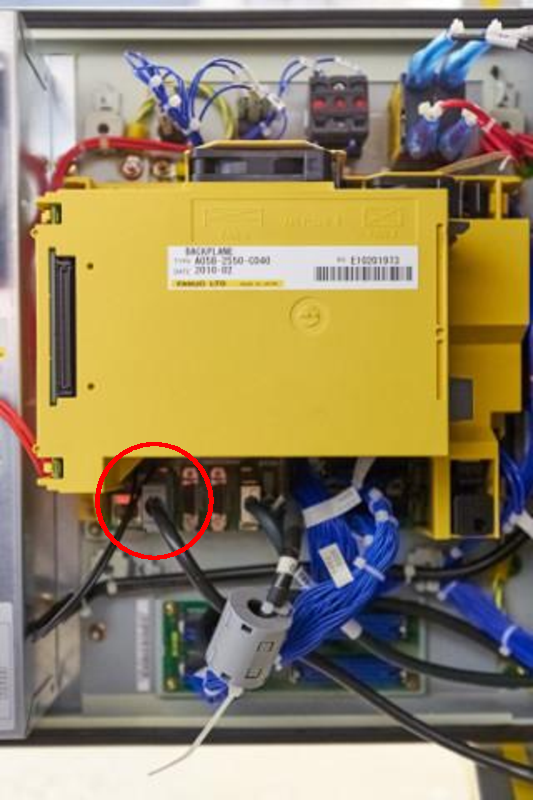
\includegraphics[width=.5\linewidth]{figures/diagrams/io-door-circled}
    \caption{I/O link cable installed in cabinet door.}
    \label{fig:io-door}
\end{figure}

\begin{figure}
    \centering
    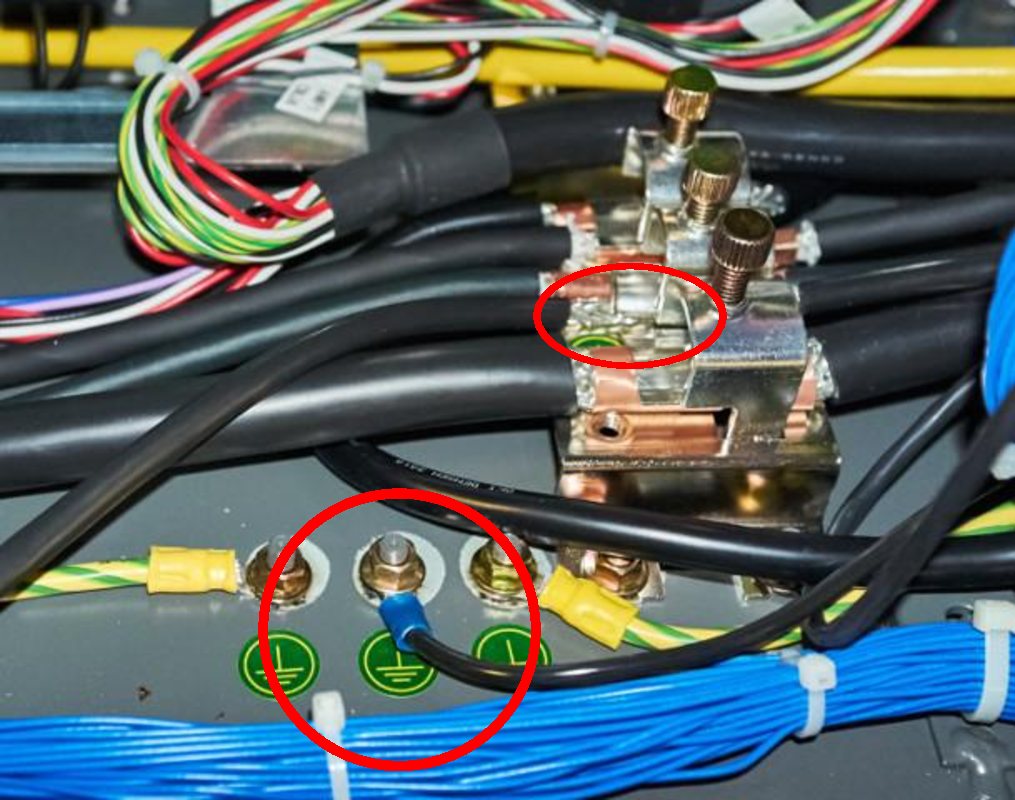
\includegraphics[width=.8\linewidth]{figures/diagrams/io-ground-circled}
    \caption{I/O link cable and back plane grounding.}
    \label{fig:io-ground}
\end{figure}

\subsubsection{Housing design}
A housing cabinet was designed and built to protect the I/O modules and allow access for maintenance and further expansion. The installed cabinet is shown in Figures~\ref{fig:cabinet1} and ~\ref{fig:cabinet2}. The cabinet was designed with inside dimensions according to \cite[sec~3.2]{io-unit}. Because the total heat generation of the two modules is only 4.3W, according to \cite[Table~3.3]{io-unit}, no special ventilation features were added. The cabinet mounts to the CERT cart frame alongside the FANUC controller. Drawings and a bill of materials for the cabinet are in \ref{sec:cabinet-drawings}.

\begin{figure}
    \centering
    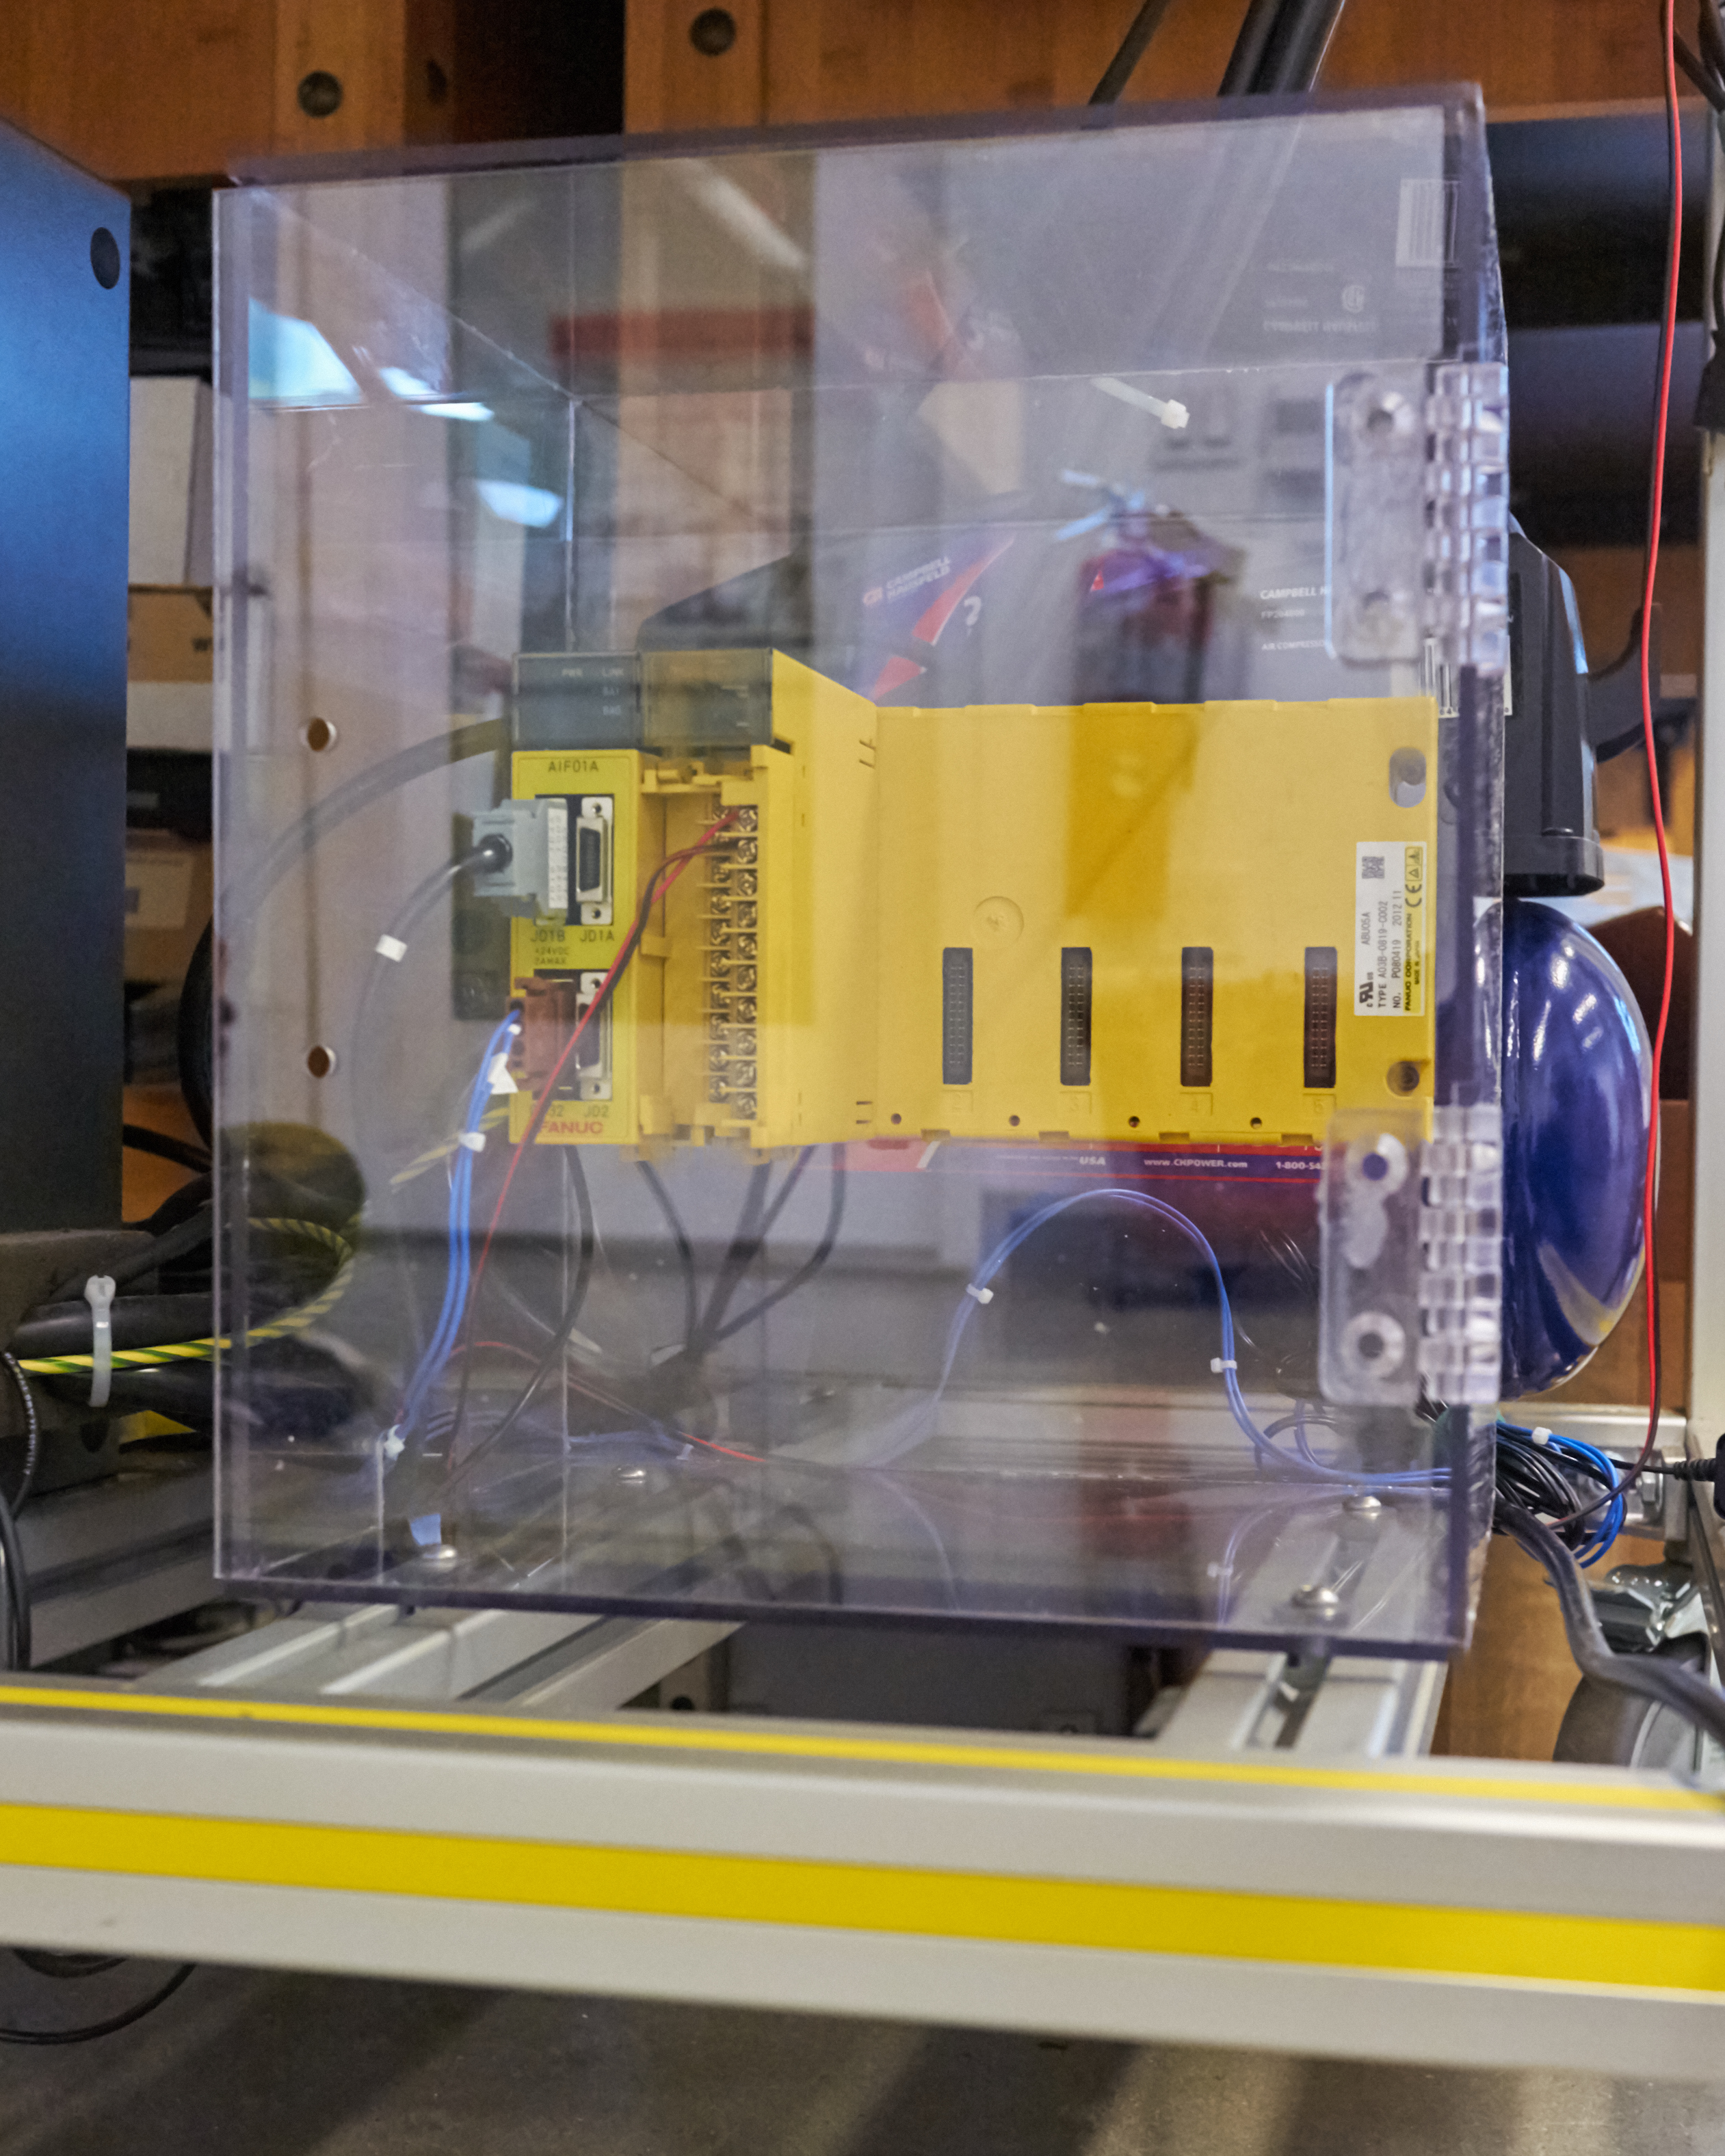
\includegraphics[width=.5\linewidth]{figures/cabinet1}
    \caption{The I/O cabinet.}
    \label{fig:cabinet-1}
    \end{figure}

\begin{figure}
    \centering
    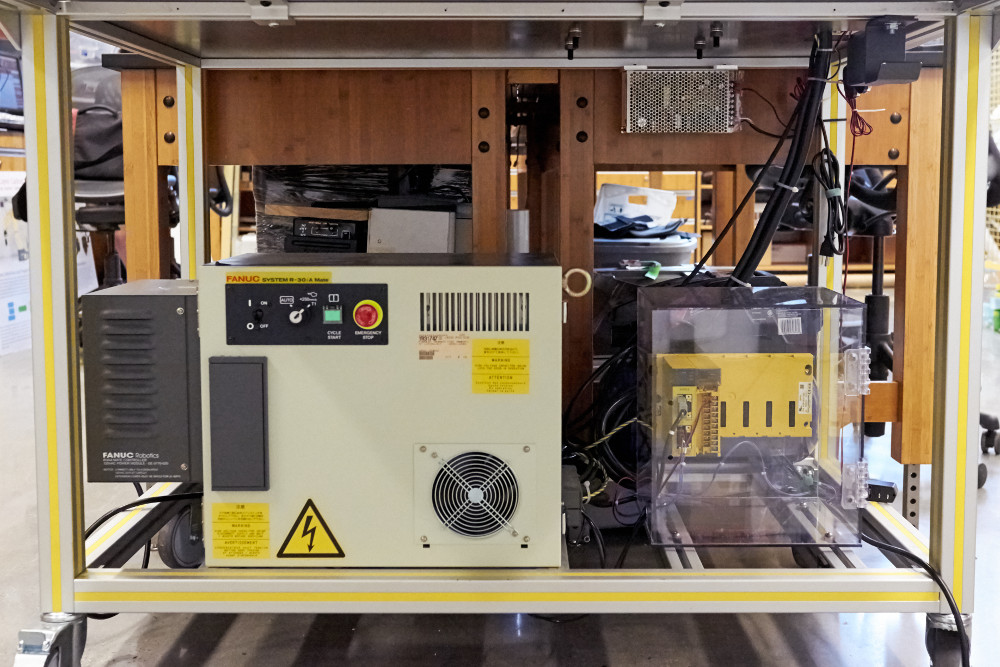
\includegraphics[width=.8\linewidth]{figures/cabinet2}
    \caption{The I/O cabinet installed alongside the FANUC controller.}
    \label{fig:cabinet-2}
\end{figure}

\subsection{Jameco power supply}
\subsection{Megatronics board}
\subsubsection{Mounting}
\subsubsection{Wiring and connections}
\subsubsection{Firmware}
